% !TeX spellcheck = ru_RU
% !TEX root = vkr.tex

\section{Обзор}

Данный раздел содержит обзор сущностей, взаимодейсвующих с глобальной очередью, метрик рантайма, инструментов бенчмаркинга.

\subsection{Многопоточный рантайм tokio}

При инстанциации рантайм создает определенное количество системных потоков для так называемого блокирующего пулла, призванного исполнять cpu bound задачи. Всего создается \verb|worker_threads| + \verb|max_blocking_threads| потков, где

\begin{itemize}
    \item \verb|worker_threads| --- количесво потоков предназначенных для исполенния асинхронных задач
    \item \verb|max_blocking_threads| --- максимальное количество блокирующих потоков
\end{itemize}

\begin{figure}[H]
    \begin{center}
        \makebox[\textwidth]{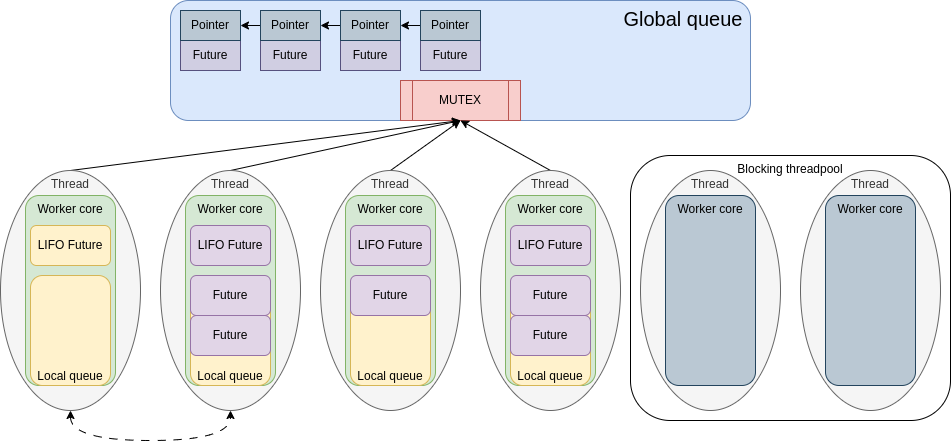
\includegraphics[scale=0.55]{pictures/tokio.arch.png}}
    \end{center}

    \caption{Упрощенное представление многопоточного рантайма}
    \label{fig:before}
\end{figure}

Блокирующие потоки ожидают определенный период, 10 секунд если не специфицировано иначе, поступления задач после чего прекращают свое исполнение.

\verb|Воркер|, так называется сущность ассоциированная с каждым из оставшихся \verb|worker_threads| потоков по средством размещения в локальной для этих поток переменной так называемого \verb|ядра воркера| --- структуры, необходимой для исполнения асинхронных задач, включающей \verb|локальную очередь|, хендлер \verb|глобальной очереди| и тому подобное.

\verb|Локальная очередь| воркера выступает в качестве кэша его задач, имеет фиксированный размер и предполагает добавление задач исключительно из потока владельца. Однако, изъятие из нее может быть осуществленно потоками других воркеров при нехватке оным собственных задач --- процесс называемый стилингом. Все это: фиксированный размер и производитель в единственном количестве позволяет ей иметь lock free алгоритм взаимодействия. В случае переполнения часть задач перемещается воркером в глобальную очередь.

\verb|Глобальная очередь| или \verb|inject queue| представляет собой коллекцию задач ожидающих исполнения. Наполняется она при спавнинге задачи вне контекста воркера или при переполеннии локальной очереди воркеров. Реализована с помощью интрузивного связного списка, защищенного мьютексом.

Исполнить асинхронное замыкание пользователь может несколькими способами:

\begin{itemize}
    \item \verb|block_on| --- метод инстанса рантайма позволяющий заблокировать поток приложения на исполнении определенного асинхронной задачи
    \item \verb|tokio::spawn| --- функция позволяющая поместить асинхронное замыкание в одну из очередей рантайма. Вызвов ее должен быть совершен в его контексте --- в одном из потоков, управляемых рантаймом, в методе \verb|block_on| или промежутке жизни объекта \verb|EnterGuard|. От места вызова будет зависеть, в какую очередь будет помещена задача: в случае потока воркер --- в локальную очередь, иначе --- глобальную
\end{itemize}

% TODO
\subsubsection{Выбор задачи}

Логика поиска воркером задачи для исполнения отражена на листинге \ref{listing:next_task}.

\begin{listing}
    \begin{minted}{rust}
fn next_task(&mut self) -> Option<Notified> {
    if self.tick % self.global_queue_interval == 0 {
        return next_remote_task()
                .or_else(|| self.next_local_task())
    }
    if Some(task) = self.next_local_task()  {
        return Some(task);
    }
    if inject().is_empty() {
        return None;
    }
    let (head, tail) = inject().pop_n(self.can_take());
    self.run_queue.push_back(tail);
    return head
}
    \end{minted}

    \caption{Логика выбора задачи}
    \label{listing:next_task}
\end{listing}

И осуществляется в следующем порядке: раз в определенное, конфигурируемое рантаймом, число тиков --- мера времени воркера, он пытается взять задачу из глобальной очереди, иначе --- из локальной, в остальное время проверяется локальная, после глобальная очереди.

\subsection{Цикл работы воркера}

Алгоритм рабочего цикла воркера отражен на листинге \ref{listing:worker:run}.

\begin{listing}
    \begin{minted}{rust}
fn run() {
    while !is_shutdown() {
        core.tick();
        if let Some(task) = core.next_task() {
            self.run_task(task, core);
            continue;
        }
        if let Some(task) = core.steal_work() {
            self.run_task(task, core);
            continue;
        }
        self.park(core)
    }
}
    \end{minted}

    \caption{Логика выбора следующей задачи}
    \label{listing:worker:run}
\end{listing}

А именно, воркер отсчиты тик, затем пытается взять найти задачу, после чего пытается украсть задачи у других воркеров. В случае неудачи он паркует поток.

\subsection{Метрики}

Метрики собираемые рантаймом предполагается использовать в двух направлениях:

\begin{itemize}
    \item Семплирование --- наблюдения поведения внутренних структур рантайма в определенный моменты исполнения задач
    \item Тотальная оценка --- анализ количеств тех или иных операций произведенных за весь период исполнения
\end{itemize}

К первому типу можно отнести глубину глобальной или локальных очередей в определенный момент времени. К последнему --- количество переполнений локальных очередей за все время исполнения. Стоит отметить, что количество переполнений без сомнений имеет смысл фиксировать и во время исполнения определенных сценариев, однако, семплинг не точен и с легкостью может упустить стремительно меняющиеся значения. Тогда как тотальная сумма не позволяет упускать отдельные опреции.

\verb|tokio-metrics| --- проект, предоставющий интерфейс для семплирования метрик рантайма. Далее будет представлен полный перечень метрик доступных из \verb|tokio-metrics|. Метрики будут разбиты на группы по аналогии для уменьшения повторений.

Группа предполагает перечисление в следующем порядке: значение представленное в tokio-metrics как общее значение для всех воркеров, минимум и максимум среди воркеров, оданко, для краткости в тексте будут обзоначены только именования суммарных.

\begin{itemize}
    \item \verb|total_park_count| --- количество парковок потоков воркеров
    \item \verb|mean_poll_duration| --- это значение представляет собой экспоненциально взвешенную скользящую среднюю продолжительности опросов задач
    \item \verb|total_noop_count| --- сколько раз поток воркера был распаркован, но не совершил никакой работы перед парковкой
    \item \verb|total_steal_count| --- количество задач, которые воркеры похитили, перместив их в свою локальную очередь
    \item \verb|total_steal_operations| --- количесво раз воркеры успешно похител задачи
    \item \verb|total_local_schedule_count| --- количество задач отправленных на исполенние из контектса воркера, что должна попасть в одну из локальных очередей
    \item \verb|total_overflow_count| --- сколько раз воркеры переполнили свои локальные очереди
    \item \verb|total_polls_count| --- количество опросов задач среди
    \item \verb|total_busy_duration| --- количество времени исполения задач
    \item \verb|total_local_queue_depth| --- количество задач помещенных в локальные очереди
\end{itemize}

И остальные:

\begin{itemize}
    \item \verb|workers_count| --- количество воркеров исполняющих задачи. Значение специфицируется при инстанциации рантайма

    \item \verb|poll_time_histogram| --- гистограмма опросов задач, сгруппированная по времени исполнения опросов

    \item \verb|num_remote_schedules| --- количество задач, отправленных на исполнение из вне. То есть количество задачи заспавненных вне контекста воркера, задач, попавших в глобальную очередь

    \item \verb|global_queue_depth| --- количество задач, помещенных в глобальную очередь
\end{itemize}

Для решения поставленных задач были выделены метрики, отражающие взаимодействие воркеров с очередями. То есть, метрики, демонстрирущие глубину глобальной очереди (\verb|global_queue_depth|), локальных очередей (\verb|total_local_queue_depth|), количество переполнений (\verb|total_overflow_count|), количество похищенных задач (\verb|total_steal_count|), количество удаленных спавнов (\verb|num_remote_schedules|).

\subsection{Бенчмаркинг}

Для измерений времени исполнения и пропускной способности была использована библиотека \verb|criterion|\footnote{\href{https://github.com/bheisler/criterion.rs}{Репозиторий} проекта criterion}. Так как она популярна, имеет обширную документацию, использовуется в \verb|tokio|.

\subsection{Изменения шедулера языка Go}

Как было отмечено ранее, алгоритмы шедулинга в tokio были созданы с оглядкой на реализацию рантайма языка Go. В свою очередь шедулинг корутин в Kotlin был сделать по мотивам tokio. С тех пор, никаких изменений рантайм Go не претерпел, точно так же, как рантайм языка Kotlin. Таким образом, все рантаймы предопологают наличия локальных очередей у воркеров и одной глобальной очереди с взаимноисключающим владением.
